\documentclass[conference]{IEEEtran}

% *** CITATION PACKAGES ***
%
%\usepackage{cite}
% cite.sty was written by Donald Arseneau
% V1.6 and later of IEEEtran pre-defines the format of the cite.sty package
% \cite{} output to follow that of the IEEE. Loading the cite package will
% result in citation numbers being automatically sorted and properly
% "compressed/ranged". e.g., [1], [9], [2], [7], [5], [6] without using
% cite.sty will become [1], [2], [5]--[7], [9] using cite.sty. cite.sty's
% \cite will automatically add leading space, if needed. Use cite.sty's
% noadjust option (cite.sty V3.8 and later) if you want to turn this off
% such as if a citation ever needs to be enclosed in parenthesis.
% cite.sty is already installed on most LaTeX systems. Be sure and use
% version 5.0 (2009-03-20) and later if using hyperref.sty.
% The latest version can be obtained at:
% http://www.ctan.org/pkg/cite
% The documentation is contained in the cite.sty file itself.

% *** GRAPHICS RELATED PACKAGES ***
%
\ifCLASSINFOpdf
  \usepackage[pdftex]{graphicx}
  \graphicspath{{img/}}
  \DeclareGraphicsExtensions{.pdf,.jpeg,.png}
\else
  % or other class option (dvipsone, dvipdf, if not using dvips). graphicx
  % will default to the driver specified in the system graphics.cfg if no
  % driver is specified.
  % \usepackage[dvips]{graphicx}
  % declare the path(s) where your graphic files are
  % \graphicspath{{../eps/}}
  % and their extensions so you won't have to specify these with
  % every instance of \includegraphics
  % \DeclareGraphicsExtensions{.eps}
\fi
% graphicx was written by David Carlisle and Sebastian Rahtz. It is
% required if you want graphics, photos, etc. graphicx.sty is already
% installed on most LaTeX systems. The latest version and documentation
% can be obtained at:
% http://www.ctan.org/pkg/graphicx
% Another good source of documentation is "Using Imported Graphics in
% LaTeX2e" by Keith Reckdahl which can be found at:
% http://www.ctan.org/pkg/epslatex
%
% latex, and pdflatex in dvi mode, support graphics in encapsulated
% postscript (.eps) format. pdflatex in pdf mode supports graphics
% in .pdf, .jpeg, .png and .mps (metapost) formats. Users should ensure
% that all non-photo figures use a vector format (.eps, .pdf, .mps) and
% not a bitmapped formats (.jpeg, .png). The IEEE frowns on bitmapped formats
% which can result in "jaggedy"/blurry rendering of lines and letters as
% well as large increases in file sizes.
%
% You can find documentation about the pdfTeX application at:
% http://www.tug.org/applications/pdftex


% *** ALIGNMENT PACKAGES ***
%
%\usepackage{array}
% Frank Mittelbach's and David Carlisle's array.sty patches and improves
% the standard LaTeX2e array and tabular environments to provide better
% appearance and additional user controls. As the default LaTeX2e table
% generation code is lacking to the point of almost being broken with
% respect to the quality of the end results, all users are strongly
% advised to use an enhanced (at the very least that provided by array.sty)
% set of table tools. array.sty is already installed on most systems. The
% latest version and documentation can be obtained at:
% http://www.ctan.org/pkg/array

% correct bad hyphenation here
\hyphenation{op-tical net-works semi-conduc-tor}

\begin{document}
%
% paper title
% Titles are generally capitalized except for words such as a, an, and, as,
% at, but, by, for, in, nor, of, on, or, the, to and up, which are usually
% not capitalized unless they are the first or last word of the title.
% Linebreaks \\ can be used within to get better formatting as desired.
% Do not put math or special symbols in the title.
\title{Towards an Automated Categorization and Rating System of Airbnb Listings in New York City}


% author names and affiliations
% use a multiple column layout for up to three different
% affiliations
\author{\IEEEauthorblockN{Jonathan Pichot, Fernando Melchor, and Avikal Somvanshi}
\IEEEauthorblockA{Center for Urban Science + Progress\\
New York University\\
New York, NY}
}

% conference papers do not typically use \thanks and this command
% is locked out in conference mode. If really needed, such as for
% the acknowledgment of grants, issue a \IEEEoverridecommandlockouts
% after \documentclass

% use for special paper notices
%\IEEEspecialpapernotice{(Invited Paper)}

% make the title area
\maketitle

% As a general rule, do not put math, special symbols or citations
% in the abstract
\begin{abstract}

\end{abstract}

\section{Introduction}
\IEEEPARstart
Airbnb is an online platform for residents of cities around the world to rent space in their homes and apartments.
Founded in 2008, Airbnb's mission is to help people "monetize their extra space." They've
been very successful, with over 3 million listings in over 65,000 cities worldwide.\cite{airbnb_about_us}
Since Airbnb listings are short-term housing provided by residents, the quality of the space
can vary drastically in quality, appointment, and amentities. The primary way Airbnb differentiates
its housing options is by the nature of the room. There are three options: shared, private, or entire home. A shared listing
is a shared space with the host, often on a couch in a living room. A private listing has
a door, usually a bedroom. And finally, a host can rent their entire home or apartment for a period of time.

Airbnb allows hosts to list the attributes of their listing, including photos, access to
technology, parking, washer/dryer, and other amentities. Past guests can leave reviews
that give further context to the quality of the place. But Airbnb does not rate the neighborhood
or location of the listing itself. For some more popular destinations, Airbnb does provide
neighborhood guides on their website.

This project will explore the possibility of creating a machine-learning driven
categorization system of Airbnb listings in New York City. A rating system similar to
the 'star rating' systems developed by the departments of tourism in several countries
is a good example of how this kind of rating system might work. This project will focus
on neighborhood attributes around a listing rather than attributes on the listing itself,
but the techniques used could be applied to listing attributes as well.

The classification system developed could be useful to tourists and Airbnb alike.
Using the system, Airbnb customers in New York City would get a better idea of the amenities available
in the neighborhood around their rental, and Airbnb could use the analysis to better understand
their listing inventory and customer preferences. Is there stronger demand for cheaper listings?
For listings with better public transit connectivity? For listings close to certain
kinds of amentities? There are several rich possible applications.

\section{Data and Methods}

\subsection{Airbnb Listings}
The Airbnb listings for New York City were collected from InsideAirbnb.com,\cite{insideairbnb} a
website run by a New York City-based housing activist named Murray Cox. The website
scrapes Airbnb's website for many cities around the world, creating snapshots of all
listings on the site in a city on a given day. The data used in this analysis was from the
scrape of New York City on March 2nd, 2017.

The scraped data includes a lot of relevant information that was used in the analysis
including the price of the listing, how many reviews have been posted on it, its
approximate location (Airbnb does not publish the exact location of listings for security
reasons), the minimum number of nights per booking, the room type (shared, private, entire), and
many more.

\subsection{Outliers}
To make sure the analysis was performed on Airbnb listings that are actually being rented we
removed certain outliers. This left us with the listings with the below attributes:

\begin{itemize}
  \item Minimum of 7 or less nights per booking
  \item Listing price of \$500 or less
  \item At least 1 review
\end{itemize}

We feel a listing requiring a booking of greater than 7 nights begins to be considered a sublet rather
than short-term housing similar to a hotel room. Some listing had absurdly high listing prices. \$500 a night
is the equivalent of a high end hotel. Finally, by requiring at least 1 review we removed
listings that had likely never been booked. After removing all outliers we end up with
28,970 listings.

\subsection{Custom Attributes}
In addition to the attributes collected by Inside Airbnb, we added four custom attributes to each listing.
We developed using publicly available data. They are:

\begin{itemize}
  \item Median Household Income
  \item Craft Beer Count
  \item Specialty Coffee Count
  \item Connectivity Score
\end{itemize}

\subsection{Median income}

\subsection{Craft Beer and Specialty Coffee Counts}
One way to disguinsh a neighborhood is to identify the kinds of businesses it can support.
Certain kinds of businesses cater to certain tastes. Two kinds of establishments that have
become popular in what could be called the 'tastemaking young professionals' class is
speciality coffee (also referred to as third-wave coffee) and craft beer. The density
of these kinds of establishments in a neighborhood should work as a good indicator of
the kind of clientele a certain neighborhood attracts.

The location of speciality coffee shops and breweries were collected using Yelp's API.\cite{yelp_api}
All coffeeshops in New York City that were returned from the API when searching for the
string 'third wave coffee' were collected. Similarly, all breweries that were returned
from the API when searching for 'brewery' were also collected. This resulted in lists of
375 coffeeshops and 67 breweries.

These lists were then run through Mapzen's Isochrone API.\cite{mapzen_isochrone} This endpoint takes a point
and returns a polygon that represents all the area one can travel to given a certain time
and using a certain mode. Every coffeeshop and brewery was then merged on a polygon that
represented the area one could access in 10 minutes while walking (also known as a walkshed).

Finally, using these walksheds, the total number of speciality coffeeshops and breweries within
a 10 minute walk was calculated for every Airbnb listing. These totals gave us what we called
our 'coffee count' and 'beer count'. The distributions of these attributes can be seen in
Figure \ref{fig_coffee_count} and Figure \ref{fig_beer_count} respectively.

\begin{figure}[!t]
\centering
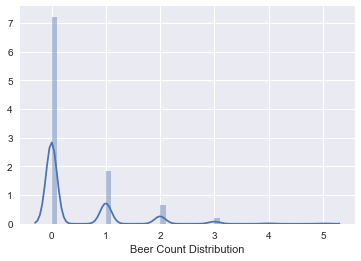
\includegraphics[width=3.5in]{beer_count}
\caption{Distribution of Beer Count}
\label{fig_beer_count}
\end{figure}

\begin{figure}[!t]
\centering
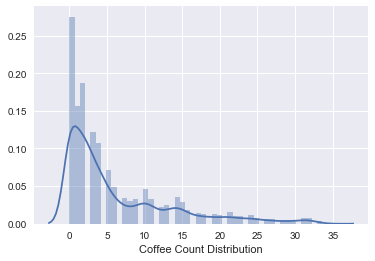
\includegraphics[width=3.5in]{coffee_count}
\caption{Distribution of Coffee Count}
\label{fig_coffee_count}
\end{figure}

\subsection{Connectivity Score}



\begin{figure}[!t]
\centering
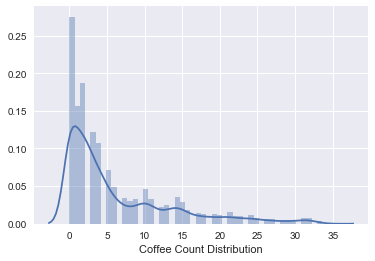
\includegraphics[width=3.5in]{coffee_count}
\caption{Asthma Hospitilization Rate per 10,000 residents}
\label{fig_coffee_count}
\end{figure}


\section{Clustering}
We

\subsection{Neighborhood Profiles}


\section{Discussion and Conclusion}


%
%\begin{figure*}[!t]
%\centering
%\subfloat[Case I]{\includegraphics[width=2.5in]{box}%
%\label{fig_first_case}}
%\hfil
%\subfloat[Case II]{\includegraphics[width=2.5in]{box}%
%\label{fig_second_case}}
%\caption{Simulation results for the network.}
%\label{fig_sim}
%\end{figure*}
%
% Note that often IEEE papers with subfigures do not employ subfigure
% captions (using the optional argument to \subfloat[]), but instead will
% reference/describe all of them (a), (b), etc., within the main caption.
% Be aware that for subfig.sty to generate the (a), (b), etc., subfigure
% labels, the optional argument to \subfloat must be present. If a
% subcaption is not desired, just leave its contents blank,
% e.g., \subfloat[].


% An example of a floating table. Note that, for IEEE style tables, the
% \caption command should come BEFORE the table and, given that table
% captions serve much like titles, are usually capitalized except for words
% such as a, an, and, as, at, but, by, for, in, nor, of, on, or, the, to
% and up, which are usually not capitalized unless they are the first or
% last word of the caption. Table text will default to \footnotesize as
% the IEEE normally uses this smaller font for tables.
% The \label must come after \caption as always.
%
%\begin{table}[!t]
%% increase table row spacing, adjust to taste
%\renewcommand{\arraystretch}{1.3}
% if using array.sty, it might be a good idea to tweak the value of
% \extrarowheight as needed to properly center the text within the cells
%\caption{An Example of a Table}
%\label{table_example}
%\centering
%% Some packages, such as MDW tools, offer better commands for making tables
%% than the plain LaTeX2e tabular which is used here.
%\begin{tabular}{|c||c|}
%\hline
%One & Two\\
%\hline
%Three & Four\\
%\hline
%\end{tabular}
%\end{table}

% trigger a \newpage just before the given reference
% number - used to balance the columns on the last page
% adjust value as needed - may need to be readjusted if
% the document is modified later
%\IEEEtriggeratref{8}
% The "triggered" command can be changed if desired:
%\IEEEtriggercmd{\enlargethispage{-5in}}

% references section

% can use a bibliography generated by BibTeX as a .bbl file
% BibTeX documentation can be easily obtained at:
% http://mirror.ctan.org/biblio/bibtex/contrib/doc/
% The IEEEtran BibTeX style support page is at:
% http://www.michaelshell.org/tex/ieeetran/bibtex/
% argument is your BibTeX string definitions and bibliography database(s)

\bibliographystyle{IEEEtran}
\bibliography{library}

% that's all folks
\end{document}
